\documentclass{llncs}
\usepackage[utf8]{inputenc}				%% Für Umlaute in UTF-8-Kodierung
\usepackage{amssymb}					%% Für alle denkbaren mathematischen Symbole
\usepackage[german,english]{babel}		%% Für deutsche (und englische) Trennungsregeln und Bezeichnungen
\usepackage{hyperref}					%% Für Hyperlinks im PDF zum Anklicken
\usepackage{apacite}					%% Für Zitationsstil gem. APA
\usepackage{graphicx}
\usepackage{amsmath}
\usepackage[linesnumbered,ruled]{algorithm2e}
\usepackage[noend]{algpseudocode}
\usepackage{acronym}
\usepackage{tocbibind}
\setcounter{secnumdepth}{3}
\setcounter{tocdepth}{3}

\begin{document}
\tableofcontents
\begin{acronym}[Bash]
	\acro{KDE}{K Desktop Environment}
	\acro{SQL}{Structured Query Language}
	\acro{Bash}{Bourne-again shell}
	\acro{JDK}{Java Development Kit}
	\acro{VM}{Virtuelle Maschine}
	\acro{CGAN}Conditional Adversarial Networks
	\acro{PIX2PIX} Image-to-Image GAN
\end{acronym}
\selectlanguage{german}
\title{3-D Datenrekonstruktion mit generative Adverserial Networks}
\author{Andreas Wiegand}
\institute{Master These in künstlicher Intelligenz}
\maketitle								%% Titel setzen
%
\begin{abstract}		
Generative Adverserial Network(GAN) ist ein kün-stliches neuronales Netzwerk(ANN) aus dem Bereich der generativen Modelle. Die Aufgabe des GANs ist es, die Wahrscheinlichkeitsverteilung von Trainingsdaten zu erlernen und dadurch anschließend neue Samples aus dieser Wahrscheinlichkeitsverteilung zu generieren. Man erhofft sich, den hohen Datenaufwand beim trainieren von ANN zu umgehen und durch GANS neue Trainingsdaten zu generieren. Im Folgenden wird auf die Theorie von GANs eingegangen, wie deren Aufbau und deren zugrunde liegendes mathematische Modell. Es wird aufgezeigt wie GANs trainiert werden. Des weiteren sollen Vorteile gegenüber anderen generativen Modelle aufgezeigt werden und derzeitige Schwachstellen von GAN, sowie Möglichkeiten diese zu verbessern.
\end{abstract}
%
\section{Einleitung}%

In den letzten Jahren haben sich im Deep Learning Bereich besonders die discriminativen Modelle hervorgehoben, welche Input Daten wie Bilder, Audio oder Text Daten zu bestimmte Klassen zuordnen. Der Grund für das steigende Interesse liegt in der niedrigen Fehlerrate bei discriminativen Aufgaben, im Vergleich zu anderen Maschine Learning Ansätzen, wie Desicion Trees oder Markov Chains\cite{Grundlagen}. Die Modelle lernen eine Funktion welche Input Daten X auf ein Klassen Label Y abbildet. Die Modelle werden dabei von ANN repräsentiert. Man kann auch sagen das Model lernt die bedingte Wahrscheinlichkeitsverteilung $P(Y|X)$ \cite{discrim}. Generative Modelle haben die Aufgabe die Wahrscheinlichkeitsverteilung von Trainingsdatendaten zu erlernen. Es lernt eine multivariate Verteilung $P(X,Y)$, was dank der Bayes Regel auch zu $P(Y|X)$ umgeformt werden kann und somit kann das Modell auch für discriminativen Aufgaben herangezogen werden. Gleichzeitig können aber neue (x,y) Paare erzeugt werden, was zu dem Ergebnis von neuen Datensätzen führt welche nicht Teil der Trainingssample sind \cite{discrim}. In diesem Paper wird speziel auf GAN, aus der Vielzahl von generativen Modellen eingegangen. Diese wurden von Goodfellow\cite{goodfellow2014} entwickelt und ebneten den Weg für Variationen, welche auf der Grundidee von GANs aufbauen. 2017 wurden alleine 227 neue Paper zu diesem Thema vorgestellt. Ein Grund weshalb GAN an Popularität gewinnt ist der, dass neuronale Netzwerke mit Zunahme der Trainingsdatenanzahl eine Erhöhung der Performance für die sie Trainiert werden zeigen. Was bedeutet,dass sich mit Zunahme der Datenanzahl die Chance auf eine bessere Performance der Neuronalen Netzwerke ergibt \cite{data}. An diesem Punkt erhofft man sich durch GANS mehr qualitative Daten zu erzeugen und somit das Trainingsergebnis zu discriminativen Modelle zu verbessern. 

\subsection{Objectives}

In den letzten Jahren haben sich im Deep Learning Bereich besonders die discriminativen Modelle hervorgehoben, welche Input Daten wie Bilder, Audio oder Text Daten zu bestimmte Klassen zuordnen. Der Grund für das steigende Interesse liegt in der niedrigen Fehlerrate bei discriminativen Aufgaben, im Vergleich zu anderen Maschine Learning Ansätzen, wie Desicion Trees oder Markov Chains\cite{Grundlagen}. Die Modelle lernen eine Funktion welche Input Daten X auf ein Klassen Label Y abbildet. Die Modelle werden dabei von ANN repräsentiert. Man kann auch sagen das Model lernt die bedingte Wahrscheinlichkeitsverteilung $P(Y|X)$ \cite{discrim}. Generative Modelle haben die Aufgabe die Wahrscheinlichkeitsverteilung von Trainingsdatendaten zu erlernen. Es lernt eine multivariate Verteilung $P(X,Y)$, was dank der Bayes Regel auch zu $P(Y|X)$ umgeformt werden kann und somit kann das Modell auch für discriminativen Aufgaben herangezogen werden. Gleichzeitig können aber neue (x,y) Paare erzeugt werden, was zu dem Ergebnis von neuen Datensätzen führt welche nicht Teil der Trainingssample sind \cite{discrim}. In diesem Paper wird speziel auf GAN, aus der Vielzahl von generativen Modellen eingegangen. Diese wurden von Goodfellow\cite{goodfellow2014} entwickelt und ebneten den Weg für Variationen, welche auf der Grundidee von GANs aufbauen. 2017 wurden alleine 227 neue Paper zu diesem Thema vorgestellt. Ein Grund weshalb GAN an Popularität gewinnt ist der, dass neuronale Netzwerke mit Zunahme der Trainingsdatenanzahl eine Erhöhung der Performance für die sie Trainiert werden zeigen. Was bedeutet,dass sich mit Zunahme der Datenanzahl die Chance auf eine bessere Performance der Neuronalen Netzwerke ergibt \cite{data}. An diesem Punkt erhofft man sich durch GANS mehr qualitative Daten zu erzeugen und somit das Trainingsergebnis zu discriminativen Modelle zu verbessern. 

\subsection{Outline}
This thesis is structured as follows Chapter 2 - Methods This chapter provides the experimental design, data set and evaluation metrics used in this thesis. Furthermore the selected approaches that are used for semantic and instance segmentation are introduced.Methods This chapter provides the experimental design, data set and evaluation metrics used in this thesis. Furthermore the selected approaches that are used for semantic and instance segmentation are introduced.Methods This chapter provides the experimental design, data set and evaluation metrics used in this thesis. 
\\\\
Chapter 3 - Methods This chapter provides the experimental design, data set and evaluation metrics used in this thesis. Furthermore the selected approaches that are used for semantic and instance segmentation are introduced.
\\\\

Chapter 4 - Methods This chapter provides the experimental design, data set and evaluation metrics used in this thesis. Furthermore the selected approaches that are used for semantic and instance segmentation are introduced. 
\\\\
Chapter 5 - Discussion The thesis ends with a discussion of the results and the limitations of this work. In addition, an outlook is given on possible research directions

\section{Grundlagen und ähnliche Arbeiten}

Im folgenden Kapitel wird auf theoretische Grundlagen eingegangen, welche zum Verständnis von GANs benötigt werden. Zunächst werden  generative Modelle im Allgemeinen vorgestellt, welche den Grundgedanken der Datengeneration für GANs aufzeigen. Darauf folgend werden Convolutional Neuronale Netzwerke vorgestellt, aus welchen GANs aufgebaut werden können, um mit Bild Daten zu arbeiten.

\subsection{Batch Normalisation}

Wie in Kapitel backpropagation Algorithums gezeigt wurde wird durch den stochstischen Gradianten Vorteile gegenüber des normalen gradianten Verfahren ergeben. Durch das der Input in jeden Layern abhängig von den vorherigen Layern abhängig. Dadurch können änderungen in vorherigen Layern große Auswirkungen in tiefern Layern im Netzwerk haben.
Dadurch resultiert dann das in trainingsläufen die Verteilung von jeden Layens input sich während des Trainings verändert die verlangsamt das Training erheblich \cite{batchnorm}. Dieses Problem wird als internal covariate shift definiert. Wenn sich die Input Verteilung von einen lernenden System verändert macht es einen covariate shift durch \cite{batchnorm}. 
Um dies zu verhindert zeigten Sergey Ioffe und Christian Szegedy \cite{batchnorm} eine Methode welche Batchnormalization genannt wird.Je mehr Layer das Netzwerk hat desto stärker wird der internal covariate shift. Batch normalization besteht aus zwei Algorithmen. Algortithmus 1 verändert den eigentlichen Input von Layer n zu einen normalisierten Input y und Algorithmus 2 verändert das eigentliche Training eine batch normalisierten Netzwerkes.

\begin{algorithm}[H]
Input: Werte von x über einen Mini-Batch $B$ = \{$x\textsubscript{1},...,x\textsubscript{n}$\}\\
\begin{math}
\mu\textsubscript{$B$}\leftarrow\frac{1}{m}\displaystyle\sum_{i=1}^{m}$x$\textsuperscript{i}
\end{math}\\
\begin{math}
\sigma\textsubscript{$B$}\leftarrow\frac{1}{m}\displaystyle\sum_{i=1}^{m}($x$\textsuperscript{i} - \mu\textsubscript{$B$})\textsuperscript{2}
\end{math}\\
\begin{math}
\hat{x\textsubscript{i}}\textsubscript{$B$}\leftarrow\frac{x\textsubscript{i}-\mu\textsubscript{$B$}}{\sqrt{\sigma\textsubscript{$B$} + \epsilon}}
\end{math}\\
\begin{math}
$y$\textsubscript{i}\leftarrow\gamma\hat{x\textsubscript{i}} + \beta \equiv BN\textsubscript{$\gamma$;$\beta$}($x$\textsubscript{i})
\end{math}\\
Output: \{$y$\textsubscript{i}=BN\textsubscript{$\gamma$;$\beta$}($x$\textsubscript{i})\}
\caption{Batch Normalisierung angewand auf x über Input bei Mini-Batch  }	
\end{algorithm}

In Schritt 2 des Algorithmus 1 wird der Erwartungswert für alle Input von Mini-Batch B berechnet. In Schritt 3 die Varianze. In Schritt 3 wird nun der der normalisierte x\textsubscript{i} berechnet welche dann mit denn $\beta$ und $\gamma$ multipliziert werden. Diese Werte sind neue gewichte im Neurnonalen Netzwerk welche während des Trainingsporcesses angepasst werden. $\epsilon$ in der Gleichung in Zeile 4 ist nur dafür da damit nicht durch 0 geteilt werden kann. In Zeile 8 - 11 werden die Inferrenz schritte beschrieben bei den der Minibatch des Trainings ersetzt wird. 

\begin{algorithm}[H]
	Input: Netzwerk N mit trainierbaren Parameter $\theta$;$\{x\textsuperscript{(k)}\}$k=1 bis 	
	\\	
	Ntr BN $\leftarrow$ N	
	\\a\\a\\a\\a\\a\\a\\a\\a\\a\\a\\

	\caption{Training mit Batch-Normalisierungs Netzwerk}	
\end{algorithm}

Schritt 1 bis 5 des Algorithmus 2 baut eigentlich nur das neuronales Netzwerk durch die transformationen aus Algorithmus 1 um. In Schritt 6 und 7 geht es darum die Parameter $\gamma$ und $\beta$ zu trainieren. Dieses passiert mit den üblichen Backpropagation Algorithmus wären des Allgemeinen Training des Netzwerkes. 


Je mehr Layer das Netzwerk hat desto stärker wird der internal covariate shift

\begin{figure}[htbp] 
	\centering
	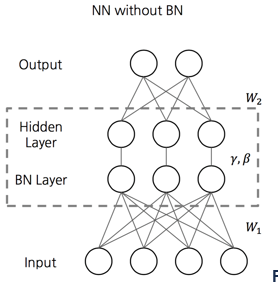
\includegraphics[width=1.0\textwidth]{batchnorm.png}
	\caption[aaaa]{Neuronales Netzwerk mit Batch Normalication Layer}
	\label{fig:Bild1}
\end{figure}

\subsection{Datenformat}
Voxel (zusammengesetzt aus dem englischen volume vox und el von elements[1]) bezeichnet in der Computergrafik einen Gitterpunkt („Bild“punkt, Datenelement) in einem dreidimensionalen Gitter. Dies entspricht einem Pixel in einem 2D-Bild, einer Rastergrafik. Wie bei Pixeln wird bei Voxeln üblicherweise die Position nicht explizit gespeichert, sondern implizit aus der Position zu anderen Voxeln hergeleitet. Im Gegensatz dazu werden bei Punkten oder Polygonen die Positionen der Eckkoordinaten gespeichert. Eine direkte Konsequenz dieses Unterschiedes ist, dass man mit Polygonen eine 3D-Struktur mit viel leerem oder homogen gefülltem Raum effizient darstellen kann. Voxel hingegen sind gut bei der Repräsentation eines äquidistant gesampelten Raums, der nicht homogen gefüllt ist. wikipedia kopie


\begin{figure}[htbp] 
	\centering
	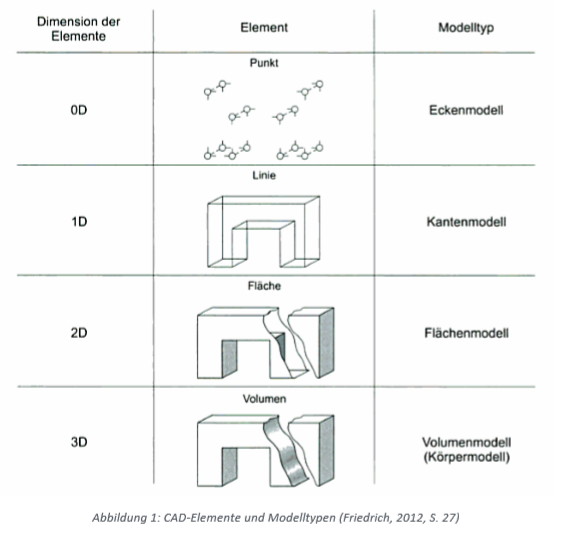
\includegraphics[width=1.0\textwidth]{datenformat.png}
	\caption{künstliches Neuron}
	\label{fig:Bild1}
\end{figure}
\subsection{Woher stammen die Daten}

Die Daten stammen von TERRA-REF Feld Scanner von der University von Arizona Maricopa Agricultural Center and USD Arid Land Researh Station in Maricopa. Es ist der größe Feld crop scnanner 
\begin{figure}[htbp] 
	\centering
	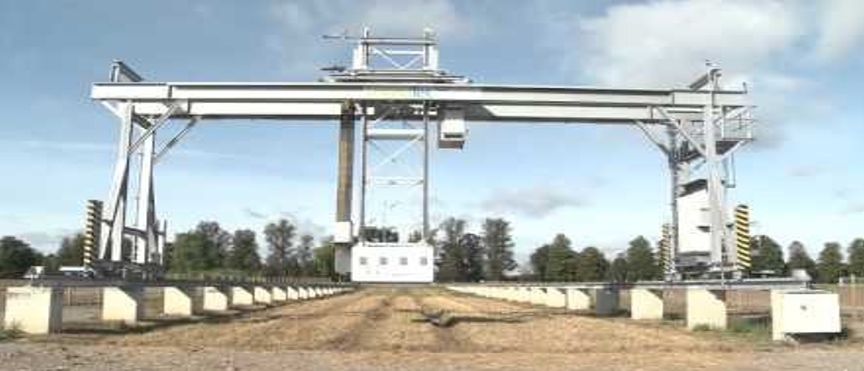
\includegraphics[width=1.0\textwidth]{lematech_1.png}
	\caption{künstliches Neuron}
	\label{fig:Bild1}
\end{figure}
\begin{figure}[htbp] 
	\centering
	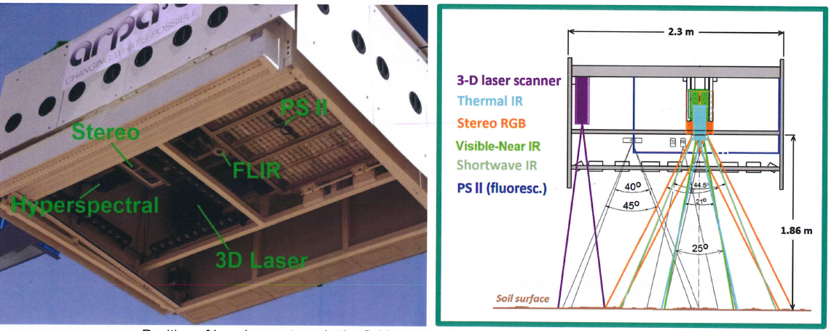
\includegraphics[width=1.0\textwidth]{lematech_2.png}
	\caption{künstliches Neuron}
	\label{fig:Bild1}
\end{figure}

\begin{tabular}{|c|c|c|c|c|c|}\hline
	Sensor & Senor Name & Beschreibung & Field of View & Pixel size(mm) & Beispiel von Potentiellen Anwendungen \\ \hline
	3D laser scanner & 3d Frauenhofer & a&a&d&b \\ \hline
	Termal IR & FLIR & a&a&d&b \\ \hline
	Stereo-RGB & Prosilica GT3300C & a&a&d&b\\ \hline
	Visual-Near IR(VNIR) & Headwall  Inspector & a&a&d&b\\ \hline
	Shortwave IR(SWIR) & Headwall Inspector & a&a&d&b\\ \hline
	PSII & PSII Camera LemmnaTec & a&a&d&b\\ \hline
\end{tabular}

Der 3D Laser Scanner erzeugt sogenannte 3D Punktwolken. Dabei werden die Objekte durch den Scanner erfasst und eine 3D Repräsentation welche durch Punkte in einen 3 Dimensionalen Koordinaten System erfasst werden können dargestellt. Dabei wird ein Laser über das zu scannende Objekt gefahren durch geflektierung des Laserstrahls auf der Oberfläche des Objektes könen x,y,z Koordinaten des jeweiligen Punktes auf den Objekt bestimmt werden.

Die Objekte werden PLY - Polygon File Format gespeichert.

\subsection{autoencoder}
Autoencoder
Autoencoder sind ein anderes Modell von generativen Modelle. Ihre Aufgabe besteht darin einen Input zu komprimieren und dann wieder zu erstellen. Die Aufgabe wird als rekunstrunktions benannt. 
Die Technik auf die Dabei zurückgegriffen wird nennt sich Dimensionreduction. Dabei werden die Dimension der Daten so reduziert und Informationen bei zu behalten welche als relevant gelten. Diese Methode finden auch in anderen Machine Learning Ansätzen Anwendung wie in beispielsweiße der Principale component anaysis(PCA). Bestandteile eines Autoencoder ist ein Encoder g parametrisiert mit $\phi$ welcher einen Input x element von $x\textsuperscript{i}$ wo x ein vektor der länge i ist. Und Damit die Input Dimension bestimmt. Dieser wird durch den Encoder auf einen Vektor $z\textsuperscript{k}$ abgebildet wobei k<i ist. Der Decoder f $\theta$ bekommt nun als Inpu t$z\textsuperscript{k}$ und mappt z auf $x\textsuperscript{l}$ wobei l = i. Und somit die gleiche Dimension wie der Input. Aufgabe ist es nun das der Encoder den Input z so gut komprimiert das encoder es schaft das x = z. 
\\\\
Die Paramter $\phi$ und $\theta$ werden durch erlernt. Und können beispielsweiße durch fully-COnnected Layer,Convolutional-Layer oder Deconvolutional Layer dargestellt werden. Eine Metrik um zu messen wie gut das Modell seine Aufgabe erfühllt könnte Beispielsweiße Cross-Entropy functionen sein.

\begin{figure}[htbp] 
	\centering
	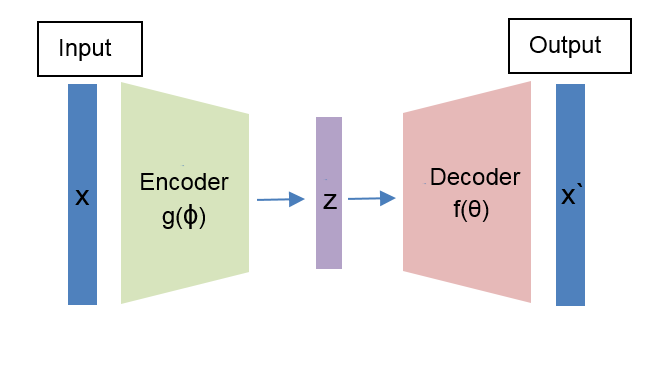
\includegraphics[width=1.0\textwidth]{autoencoder.png}
	\caption{autoencoder}
	\label{fig:Bild1}
\end{figure}

\subsubsection{Zielfunktion Autoencoder\\\\}

Da in der Arbeit der Input 3d Pointcloud sind und diese Sets und diese invariant zu ihren Permutationen. Das heißt ändere ich die Anordnung meiner einzelnen Punkte in meien Set bleibt das Ergebniss unverändert.  sind sind kann auf übliche Zielfunktionen nicht zürockgegriffen werden da diese mit Sturcturierten Input Daten arbeiten. Das Problem dabei besteht wenn ich 2 unterschiedliche Sets von Punkten habe wie Messe ich um herraus zu finden wie hoch die discrepanc zwischen den Beiden sets ist. 
http://graphics.stanford.edu/courses/cs468-17-spring/LectureSlides/L14%20-%203d%20deep%20learning%20on%20point%20cloud%20representation%20(analysis).pdf


\subsection{Objekterkennung}
Das zweite Modell beruht auf dem Konzept, der Objekterkennung auf Bildern aus den Be-reich Computer Vision. Dabei bekommt das Neuronales Netz (NN) als Input ein Bild und gibt als Output die Bounding-Box Koordinaten und die Klassenbezeichnung des Objekts mit den jeweiligen Prozentangaben zurück.
\begin{figure}[htbp] 
	\centering
	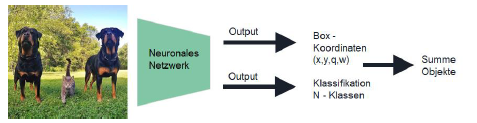
\includegraphics[width=1.0\textwidth]{objekterkennung1.png}
	\caption{künstliches Neuron}
	\label{fig:Bild1}
\end{figure}

 Im Abbildung 5-1 wird dieser Vorgang Illustriert. Der Output des NN wird in Abbildung 5-2 gezeigt.Bounding-Box Koordinaten sind vier Punkte, welche durch x und y Koordinaten auf dem Bild definiert werden. Diese Punkte kennzeichnen dann den Rahmen, welcher um das zu erkennende Objekt gelegt wird (Ross Girshick, 2014).
\begin{figure}[htbp] 
	\centering
	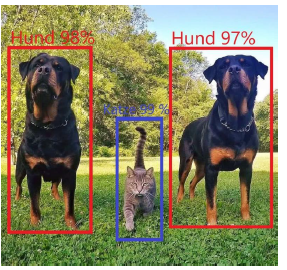
\includegraphics[width=1.0\textwidth]{objekterkennung2.png}
	\caption{künstliches Neuron}
	\label{fig:Bild1}
\end{figure}
 
Nachdem die Objekte auf dem Bild erkannt worden sind, können die einzelnen Objektklas-sen auf den Bildern aufsummiert werden. In unseren Versuchsaufbau wird ein Faster Re-gion-based Convolutional Neural Network (Faster R-CNN) eingesetzt. Die Funktionsweise des Faster R-CNN wird in Punkt „5.1.4 Faster R-CNN“ genauer erklärt. In „5.1 Stand der Forschung Objekterkennung mit NN“ wird auf die Entwicklung hin zum Faster R-CNN ein-gegangen. Der genauere Projektversuchsaufbau wird unter „5.2 Versuchsaufbau“ erläutert.
 
Um einen genaueren Einblick und das Verständnis für die Objekterkennung mit NN zu schaffen wird zunächst auf die Entwicklung in diesen Bereich eingegangen. Im Allgemeinen arbeiten NN in der Objekterkennung mit den gleichen Layern wie in „2.5 Modellierung neu-ronaler Netzwerke (Dennis Groß)“ beschrieben. Die Convolutional Layer identifizieren Fea-tures welche die Objektklassen unterscheiden. Der Pooling Layer hilft bei der Dimension Reduzierung und dadurch eine Aggregation von Features. Jegliche die Zusammensetzung der Layer und die Anzahl unterscheiden sich.
Es gibt mehre Ansätze im Deep Learning Spektrum zur Objekterkennung, beispielsweise YOLO. In diesen Versuchsaufbau wurde Faster R-CNN Modell entschieden da es mehr Ob-jekte auf einem einzigen Bild erkennen kann als YOLO. In dem folgenden Kapitel wird ein Augenmerk auf die stetigen Veränderungen im Aufbau der R-CNN Reihe und die dadurch resultierenden Verbesserungen geworfen werden (Joseph Redmon, 2016).

Selective Search bildet die Grundlage für R-CNN. Eine komplette Ausarbeitung des Algo-rithmus würde das Ziel dieser Arbeit verfehlen. Es soll lediglich das Grundkonzept veran-schaulicht werden um den Leser das Prinzip näher zu bringen. Dieser Algorithmus arbeitet nach dem Prinzip des Clustering und bildet Cluster in Pixelregion, welche im ähnliche Werte haben. Das bedeutet Pixel – die in einem definierten Skalenbereich zueinander liegen – wer-den als Gruppe zusammengefasst und anschließend mit Bounding-Boxen umrandet. Siehe Abbildung 5-3 veranschaulicht das Prinzip.Der Algorithmus hilft Bilder vorzubereiten und den Suchraum für die NN zu verkleinern, da diese später als Vorhersagen im Training genutzt werden können. Selective Search bietet den Vorteil gegenüber dem Brute Force Ansatz, dass der Suchraum der potentiellen Objekte eingeschränkt wird (R.R. Uijlings, 2012)
Der Brute Force Ansatz ist alle möglichen Region Proposal zu erstellen. In einem Fall von einen 128 x 128 Pixel Bild wären das Möglichkeiten Region Proposals.
Das Region-Based Convolutional Neural Network (R-CNN) besteht aus drei Modulen. Das Region Proposal-, Feature Extraktion-, und Classification Regions Modul, deren Komposi-tion kann in Abbildung 5-4 entnommen werden. Das Netzwerk folgt die unter –5 Objekter-kennung – Modell (Wiegand) – Modell genannten Grundzügen der Objekterkennung (Ross Girshick, 2014).
Das Prinzip von Region Proposal wurde in „5.1.1 Region Proposal – Selective Search“ er-läutert. R-CNN nutzt diesen Algorithmus um mögliche Objekte auf Bilder vorzuselektieren. Es unterteil das jeweilige Bild in bis zu 2000 Regionen, welche als Fundament für die Ob-jekterkennung gelten und gibt diese einzelnen Regionen an das Feature Extraktion Modul weiter. Dieses ist mit ähnlichen Layern aufgebaut wie das Modul in „4.1 Aufbau des neuro-nalen Netzwerks“ beschrieben. Es besteht aus mehreren darauffolgenden Convolutional Layern und Pooling Layern, gefolgt von zwei Fully-Connected Layern. Diese folgen den gleichen Prinzip, Features auf Bildern zu lernen, welche bei der Inferenz helfen bestimmte Objektklassen zu identifizieren. Dabei werden im Training die Gewichte der Sliding-Windows in den Convolutional Layer so angepasst, um objekttypische Feature zu erkennen (Ross Girshick, 2014).
Die Klassifikation erfolge über Support Vector Machines (SVM). Dabei muss vor dem Trai-ning des R-CNN festlegen werden wie viele Objektklassen der Datensatz enthält und dem-entsprechend ist die Anzahl der SVM anzupassen (Ross Girshick, 2014).
Das Ziel der Bounding Box Regression ist es, anstatt wie bei den Klassifikationsaufgaben im Deep Learning Bereich, ein stetige Variable vorherzusagen. In diesen Fall vier stetige reale Zahlen, welche die Koordinaten der Bounding Boxes darstellen. Der Input im Trai-ningsdurchlauf ist diese stehen für die vier Eckpunkte der vorhergesagten Bounding-Box Coordinaten der Selective Search. Die Koor-dinaten der Bounding Box aus den Trainingsdaten entsprechen G 
Das Ziel ist es am Ende durch die Methode – des kleinsten Quadrats – den Abstand zwischen P und G zu verkleinern. Hervorzuheben sei noch die Zuordnung, von G zu dem entsprechen-den P. Da 2000 P durch den Region Proposal Algorithmus erzeugt werden, muss entschieden werden, welches der P am ehesten eine Vorhersage für die G Koordinate liefert. Dies wird
5 Objekterkennung – Modell (Wiegand)
24
dadurch erlangt indem die Flächen der einzelnen P`s und G`s Bounding Boxes ausrechnet wird und vergleichen wird mit wieviel Prozent das jeweilige P von G abgedeckt wird. Alle P`s, welche über einen prozentualen Flächenanteil von 60% liegen, werden als Region Proposal zum G hergenommen. Die R-CNN Modell Reihe folgen einem ähnlichen Prinzip der Bounding-Box Regression. Lediglich der Aufbau der cost function unterschiedet sich (Ross Girshick, 2014).
R-CNN hat schwächen, welche durch Fast R-CNN verbessert werden. Das Training ist eine Multi-stage Pipeline. Das heißt die Bilder werden nach dem Selective Search in unter Bilder zerlegt und erst dann einzeln in das Netzwerk gegeben. Daraus resultierten eine erhöhte Trainingszeit und ein Verlust von Information, wenn man bedenkt, dass die Region Propo-sals aus den Bildern herausgeschnitten werden und in das NN nacheinander zufällig einge-speist werden.
Ein weiterer Nachteil ist der hohe Trainingsaufwand bezüglich Zeit und Speicher. Dadurch das jedes Bild durch Selektive Search in 2000 Region Proposal zerlegt wird und diese ein-zeln das Netzwerk durchlaufen, müssen jede Objekt Vorhersage und die dazugehörigen Fea-tures abgespeichert werden. Dies kann bei großen Datensätzen wie bei „VGG16“ mehrere 100 GB Speicher beanspruchen. Außerdem beträgt die Inferenzzeit bei Bildern um die 47 Sekunden pro Bild (Ross Girshick, 2014).
Das „Fast R-CNN“ von Ross Girshick baut auf das Modell „R-CNN“ auf und geht auf die in „5.1.2 R-CNN“ beschriebenen Nachteile ein. Der Aufbau kann Abbildung 5-5 entnommen werden.
5 Objekterkennung – Modell (Wiegand)
25
Abbildung 5-5 Fast R-CNN (Girshick, 2015)
Ein großer Vorteil des Modells besteht darin, dass das NN zunächst die Feature Extraktion durch die Convolution-Layers durchgeführt und dann das Region-Proposal auf die Convo-lution Feature Map durchgeführt wird. Das bedeutet, dass das Trainingsbild nicht zunächst wie in R-CNN Modell in 2000 Bilder zerlegt und in das NN geladen wird, sondern die Fea-tureextraktion das gesamte Bild durchläuft. Um die Region Proposals auf die Convolution Feature Map zu übertragen, wird ein neuer Layer namens Region of Interest Pooling Layer (ROI-Pooling) eingeführt (ROI-Pooling) (Girshick, 2015).
Das Faster R-CNN ist derzeit der aktuellste Entwicklungsstand der R-CNN Modell Reihe und wird in unserem Versuchsaufbau verwendet. In diesen wird das Region Proposal Modul durch ein Region Proposal Network abgelöst. Dieses wird durch ein NN, welches als Input die Convolutional Feature Map erhält und als Output die Region Proposal in Form von Bounding Boxes wieder an den ROI Pooling Layer weitergibt. Die Abbildung 5.7 veran-schaulicht diesen Aufbau. Dieser übernimmt die komplette Objekterkennung durch ein NN. Der daraus resultierende Vorteil ist ein durchgängig trainierbares Modell und wird durch ein Ähnliches Verfahren wie in Punkt 2.4 Gradient-Descent beschrieben realisiert (Shaoqing Ren, 2016).Das Region Proposal Network bekommt als Inputs zum einem, den Output aus den Convo-lution Layers generierten Feature Map und zum anderem k Anchor Boxes. Diese sind in einer fixierten rechteckigen Größe. Diese folgen dem gleichen Prinzip der Bounding-Boxes, welche in „5.1.2 R-CNN“ beschrieben worden sind. K Region Proposal Koordinaten sollen erzeugt werden. Anchor Boxen geben außerdem die Relationen von Länge zu Breite der Sliding-Windons vor, welche auf der Convolution Feature Map angewendet wird. Im Paper wird die Aufgabe das Netzwerk als „Attention“ beschrieben, welche für das NN den Focus
5 Objekterkennung – Modell (Wiegand)
27
auf bestimmte Bildbereiche lenkt. Die cost function für das Region Proposal Network ist zum einem geben aus, Klassifikation Region Proposal und Regression, welche die Koordi-naten mit den Ground-Truth Koordinaten der Boxen vergleicht. Die cost function folgt dem gleichen Prinzip der Bounding-Box Regression des R-CNN. Anschließend geht das Verfah-ren wie beim Fast-RCNN Modell weiter. Die vom RPN ermittelten Koordinaten werden nun auf der Convolutional Feature Map angewandt, darauf folgt das ROI-Pooling und die Klas-sifikation der einzelnen Bounding Boxen. Die dadurch resultierte Inferenzzeit ist enorm ge-stiegen und liegt im Durchschnitt bei 10 ms pro Bild (Shaoqing Ren, 2016).

\subsection{Maschine Learning Basics}
Im folgenden wird auf Grundlegende Begriffe des machines Learnings eingangen ihre Definitionen und ihr gebraucht in dieser Arbeit. Ziel ist es die Begriffe zu Definierne um keine verwirrung zu stiften. 
\newpage
\subsubsection{Überwachtes Lernen}

Der Datensatz der erlernt werden soll enthält Features welche zu einen Label oder Ziel verbunden sind. Zum Beispiel einen Datensatz welcher Rötgenbilder von Organen welche mit Label versehen sind wie "Krebs" "kein Krebs". 

\subsubsection{Unüberwachtes Lernen}

Beim unüberwachten Lernen ist das ein Datensatz mit Featuren gegeben. Ziel ist es nun die Struktur des Datensatzes zu erlernen und ihre zugrundeliegende Datenverteilung. 
\\

\subsection{Die unterschiedlichen Aufgabengebiete im Maschine Learning}

Machine Learning kann in verschiedene Aufgaben angewendet werden. Beispielsweise Klassifikation bei der ein Input X einem Label Y zugewissen wird. Anwendung kann dieses Anwenundung in Bereich Robotics bei der Klassifikation von Objekten mit dennen der Ropoter aufgaben ausführen soll. Oder bei der Bilderkennung. Synthesis und Sampling hat der Maschine Learning Algorithmus Daten zu erzeugen welche ähnlich zu den vorhanden Trainingsdaten sind. Diese Anwenundung kann Zielführent bei Aufgaben sein welche eine hohen Datenanzahl brauchen und kann beispielsweiße unterstüzent bei der Aufgaben von Klassifikationen sein. transformation hat die Aufgabe ein Bestimmten Input X zu einem Output Y umzuwandeln. Die umwandlung geschieht dabei durch bestimmte regeln \cite{dcgan}. Beispiele dafür könnte sein Bilder so umzuwandeln das sie heller oder dunkler sind oder Inhalte auf den Bilder verändert. Ein anderes Beispiel könnte sein das Texte aus einer Sprache in eine Andere übersetzt werden. 
\\
Diese Arbeit benutzt alle oben aufgezählten techniken um das Ziel zu erreichen Daten zu Transformieren dabei sythesiren und neue Samples zu generieren. Dabei gehst es darum für einen weiteren Schritt des Klassifizieren neue daten zu generieren. 



\subsection{Deep Feedforward neuroal Networks}

Künstliche Neuronale Netzwerke(ANN) haben das Ziel ein Funktion f* zu approximieren. Dabei werden Parameter $\Theta$ eines Models so angepasst, um die Abbildung von y = f(x;$\Theta)$ zu approximieren. Die Modelle werden als feedforward betitelt weil der Informationsfluss des Models von Input zu Output fließt und keine Recurrsion von Output zu Input statt findet. Deep weil das Modell aus mehrer Schichten sogenannten hidden layer besteht. Es gibt den Input layer welche den Input in das Netzwerk aufnimmt und der letzte layer des Netzwerkes wird output Layer genannt\cite{Grundlagen}. 

\begin{figure}[htbp] 
	\centering
	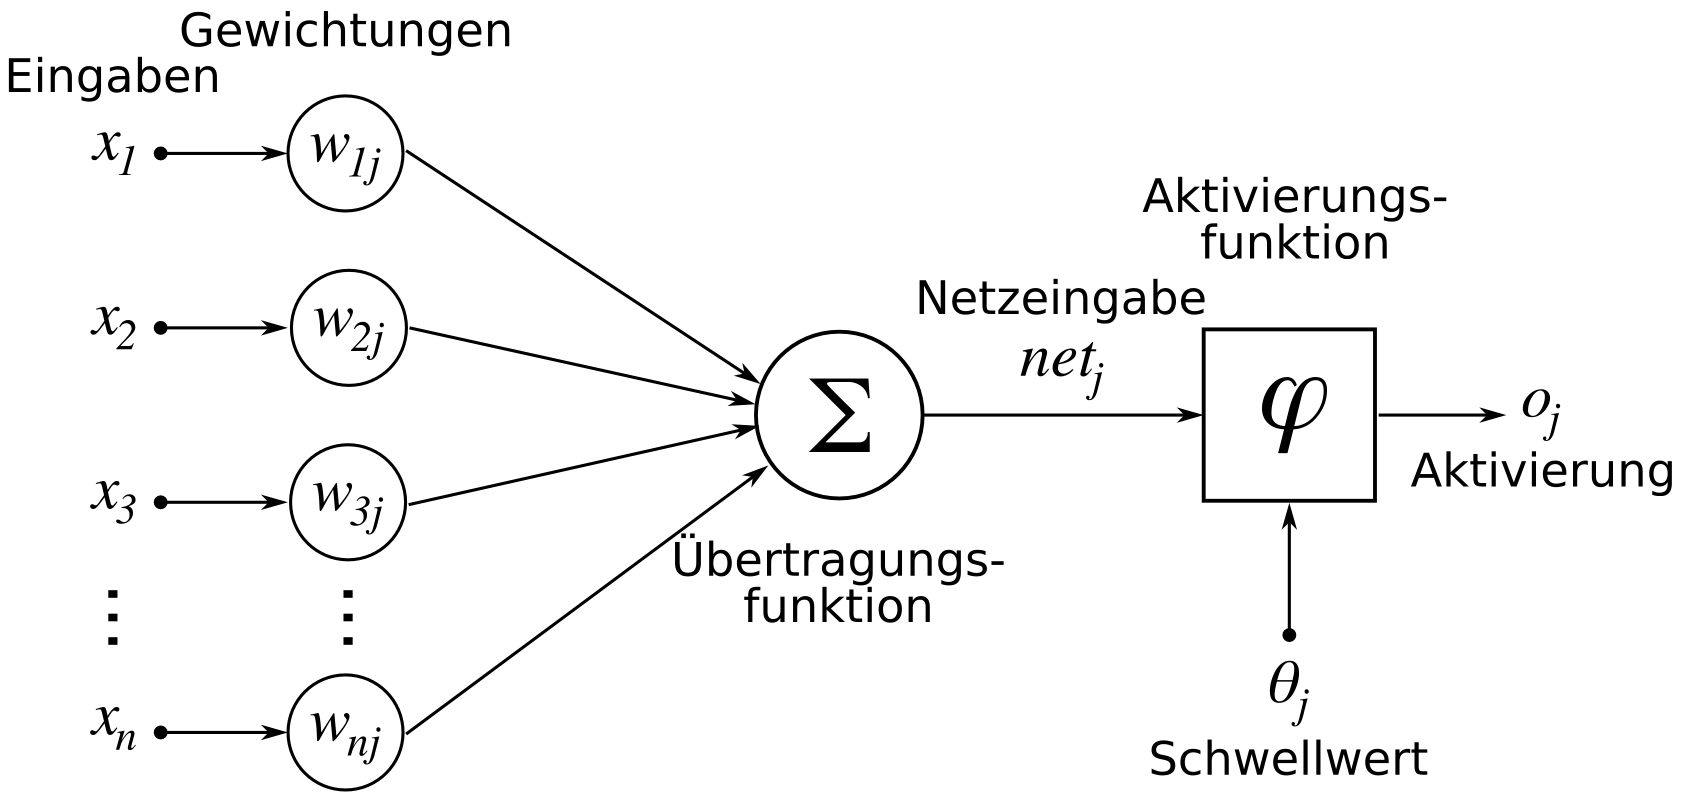
\includegraphics[width=1.0\textwidth]{Neuron.png}
	\caption{künstliches Neuron}
	\label{fig:Bild1}
\end{figure}

künstliche Neuronen haben ihren Namesgeber von der aus der natur stammende Neuron. Neuronen sind die Buasteine aus denen die Gehirne von Lebewesen, wie Fische, Vögel, Säugetiere zusammen gesetzt sind. Neuronen oder auch Nervenzellen bestehen in eine Zellkern der Zetrum der Zelle um sie herum sind dendriten. Neuronen sind untereinander mit den Axon verbunden.axon haben an den enden Synapen welche die grenze von Axon zur Nervenzelle einen Spalt bilde. Dieser Spalt überwunden indem von der Synapse botenstoffe abgesendet werden welche sich dann an Rezeptor der Zelle anhaften. Diese Übertragung findet statt wenn an der Synapse ein bestimmter Schwellenwert überschritten wurde von elektrischen reizen welche die Zelle abfeurt lässt. Künstliche Neuronen haben diese Schwellenwert durch songenannte Gewichte w\textsubscript{ij} diese sind auf den Verbidungen zwischen den Neuronen in den unterschiedlichen layern im Netwerk
\begin{figure}[htbp] 
	\centering
	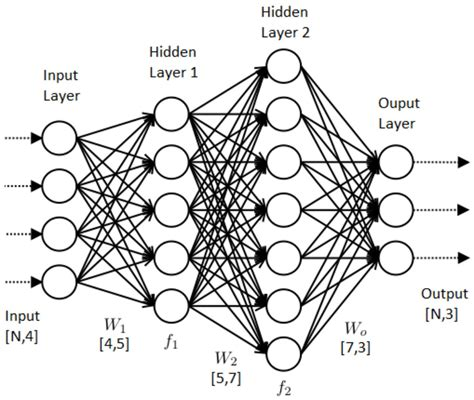
\includegraphics[width=1.0\textwidth]{neuronalesnetzwerk.jpg}
	\caption{künstliches neuronales Netzwerk}
	\label{fig:Bild1}
\end{figure}
\\

\subsection{Backpropagation Algogrithmus}
Wurde von Geofrey Hintion im Jahre 1989 vorgestellt\cite{backpro}. Er konnte zeigen das sein Algorithmus schneller und effizienter auf Neuronalen Networks arbeitet als andere vor ihm. Das mathematische Zugrundeliegende Konzept ist die der Partitiellen Ableitung von  $\frac{\partial Z}{\partial w}$, wobei Z die Zielfunktion und w die Gewichte im zu Optimierenden Neuronalen Netzwerk sind. Für eine Funktion $f$(x) = y ist die Ableitung Definiert als $f^\prime$(x) oder $\frac{dy}{dx}$ und gibt die Steigung der Funktion an Punkt x an. Dieses Verfahren kann dabei helfen Funktionen zu optimieren. Wenn man weiß wie sehr die Steigung and Punkt x ist kann man x mit einer Änderung von der Ableitung x dahin gehen optimieren \cite{Grundlagen}. \\
Wenn nun $f^\prime$(x) = 0 haben wir keinerlei Information über die Steigung erreicht. Dies ist aber kein garant dafür das $f$ ein Optimum erreicht hat.  Es könnten wie in Abbildung unten dargstellt. Ein locales Minimum sein. Dass heißt das wir nur an diesen Punkt ein Minimum erreich thaben aber im Funktionsverlauf ein noch niedrigeres Minimum vorhanden ist. Oder einen Sattlepunkt welche ein Übergang zu einen anstieg der Funktion bildet.
Ist nun die die Funktion $f$ definiert als $f$: $\mathbb{R}$\textsuperscript{n} $\rightarrow$  $\mathbb{R}$ und hat als Input mehrere Variablen. Die partielle Ableitung $\frac{\partial f(x)}{\partial x\textsubscript{i}}$ zeigt an wie sehr sich $f(x)$ ändert wenn wir x\textsubscript{i} ändern. Der Gradiant $\nabla\textsubscript{x}f(x)$ ist ein Vektor welche alle partiellen Ableitungen von $f$ enthält. Nun kann man f optimierne in dem man in die Richtung des Gradianten geht welche negativ ist dieses Verfahren wird gradient descent genannt \cite{Grundlagen}.
\begin{figure}[htbp] 
	\centering
	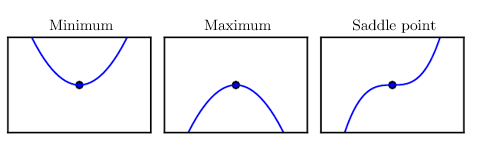
\includegraphics[width=1.0\textwidth]{saddle.png}
	\caption{Minimum Maximum Saddle Point}
	\label{fig:Bild1}
\end{figure}


Algorithmen die für Deep Learning eingesetzt werden, beinhalten eine Art von Optimierung, ohne diese ist eine Umsetzung des Lernprozesses nahezu unmöglich. Diese Minimierungs-funktionen oder auch cost function (welche in vielen Publikationen unterschiedlich bezeich-net wird „loss“- oder „error function“) wollen immer dasselbe Ziel: eine gewisse Target Funktion ermitteln, welche für einen Input den gewünschten Output ausgibt. Das Ziel ist in anderen Worten eine Menge an Gewichten und Biases zu finden, für welche, die quadrati-schen Kosten (C(w,b)) so gering wie möglich sind. Um dies zu erreichen, wird der Gradient Decient Algorithmus eingesetzt (Nielsen, 2017).
Der Grund des Einsatzes dieses Algorithmus ist derer, dass zwar versucht werden könnte die Anzahl der richtig klassifizierten Bilder direkt zu erhöhen. Aber das Problem ist, den Per-formancegewinn bei Veränderungen der Gewichte festzustellen. Da meisten kleine Verän-derungen an den Gewichten und Baises führen zu keinerlei Veränderung bei der Klassifizie-rung. Somit liegt eine gewisse Schwierigkeit, bei der Ermittlung der richtigen Anpassung dieser Werte. Zuerst muss die quadratische cost function (C (w,b)) minimiert werden, bevor sich die Maximierung der Bestimmungsgenauigkeit des Netzwerkes als Ziel gesetzt kann (Nielsen, 2017).
\begin{figure}[htbp] 
	\centering
	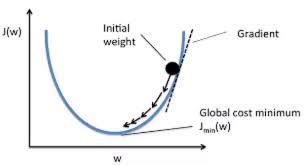
\includegraphics[width=1.0\textwidth]{gradient.png}
	\caption{LossFunktion}
	\label{fig:Bild1}
\end{figure}

Backpropagation Algorithmus wird das Verfahren genannt mit den ANN trainiert werden. Dabei wird der Gradiant der Ziel Funktion bestimmt.

\subsubsection{momentum}
Momentum hat das Ziel das Gradientenverfahren zu beschleunigen  um eine effizienter Konfergierung der Zielfunktion herbei zu führen und ein schnelleres Lernen erzielt. 

\begin{math}
\\\\
v\textsubscript{t+1} =\mu v\textsubscript{t}-\epsilon\nabla$f$(\theta\textsubscript{t})
\\
\theta\textsubscript{t+1}= \theta\textsubscript{t}+v\textsubscript{t+1}
\\\
\end{math}

wobei $\epsilon$ $>$ 0 die Lernrate ist und $\mu$ $\in$ [0,1] das Momentum ist und $\nabla$f$(\theta\textsubscript{t}$ der Gradiant von $\theta\textsubscript{t}$ ist. Je größter das Momentum desto schneller Bewegt sich der Gradient abwärts. Da am Anfang eines Lernphase der gradiant überlicherweiße recht hoch ist empfielt sich zunächst mit einen niedrigen Momentum zu Arbeiten da sonnst die Gefahr besteht über das globale Optimum hinüberzuschießen. Wenn nun das Training stagniert welches auf Gründe der Aufbau der Loss-Funktion zurückzuführen ist das zur nähe des globalen Optimums flache Täller entstehen welche das Trainings verlangsamen. und es zu keiner Verbesserung kommt kann man durch momentum erzwingen größere Gradianten sprünge einzugehen und sich somit schneller zu einen globalen Optimum zu bewegen oder aber aus einen localen Optimum hinaus richtung eines globalen Optimum\cite{momentum}. .
\\\\\\
Here’s a popular story about momentum gradient descent is a man walking down a hill. He follows the steepest path downwards; his progress is slow, but steady. Momentum is a heavy ball rolling down the same hill. The added inertia acts both as a smoother and an accelerator, dampening oscillations and causing us to barrel through narrow valleys, small humps and local minima. 
This standard story isn’t wrong, but it fails to explain many important behaviors of momentum. In fact, momentum can be understood far more precisely if we study it on the right model. 
One nice model is the convex quadratic. This model is rich enough to reproduce momentum’s local dynamics in real problems, and yet simple enough to be understood in closed form. This balance gives us powerful traction for understanding this algorithm\cite{momentum}. 

For a step-size small enough, gradient descent makes a monotonic improvement at every iteration. It always converges, albeit to a local minimum. And under a few weak curvature conditions it can even get there at an exponential rate. 

https://distill.pub/2017/momentum/
\subsection{Nicht Lineare Gleichungssysteme}
Neurnonale Netzwerke sind universelle Funktions approximierer \cite{universal}. Es sei erfohrzuheben das zwar Feedforward Neuronale Netzwerke mit hidden Layer unisversel sind. Aber nicht jede aktivierungsfunktion ist für alle probleme gleich effizient. \cite{universal}.
In Kapital BLABLA wurde gezeigt das Neuronale Netzwerke durch Matrizen dargestellt werden können und das durch simple Matrixmultiplikation der Output von Layern berechnet werden können. Die Aktivierungsfunktion sorgen dafür das das ANN auch nicht lineare Funktionen erlernen kann. Also das unser Input X und unser Output Y immer proportional als Y = X$*$k. Wobei k eine Konstante ist.  Wie wir in Kapitel BLABLA gesehen habe möchten wir das unser Input linear Trennpaar ist damit wir unsere Input in Klassen einteilen können. Würde X nun aber nicht linear trennbar sein wie Beispielsweiße in Abbildung UNTEN gezeigt Könnten wir duch die lineare transformation des Inputs keine Trennung von X erreichen. http://colah.github.io/posts/2014-03-NN-Manifolds-Topology/ Mit den einführen von nicht linearen Funktionen können der Raum der durch die Layer dargsetllt wird gedreht gewendet und gezogen werden. Aber es scheidet, zerbricht oder faltet in. 


\begin{figure}[htbp] 
	\centering
	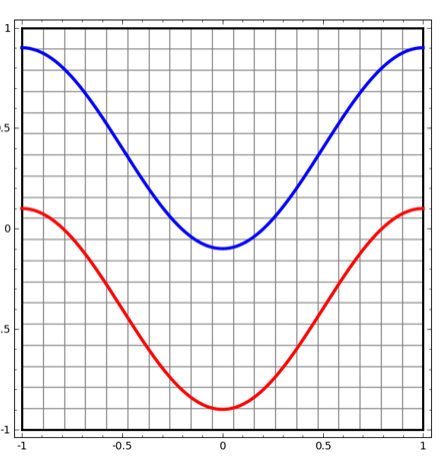
\includegraphics[width=1.0\textwidth]{lineartrennbar.png}
	\caption{Nicht trennbar}
	\label{fig:Bild1}
\end{figure}

\begin{figure}[htbp] 
	\centering
	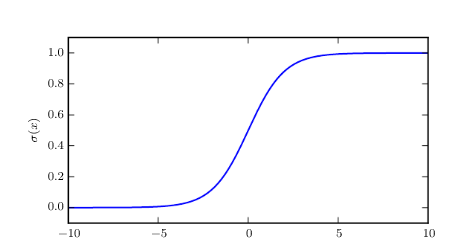
\includegraphics[width=1.0\textwidth]{sigmoid.png}
	\caption{Sigmoid Funktion}
	\label{fig:Bild1}
\end{figure}

\begin{math}
\sigma(x)=\frac{1}{1+exp(-x)}
\end{math}

\begin{figure}[htbp] 
	\centering
	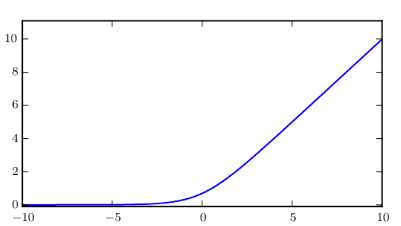
\includegraphics[width=1.0\textwidth]{softmax.png}
	\caption{Softmax}
	\label{fig:Bild1}
\end{figure}

\begin{math}
\zeta(x) = \log(1+exp(x))
\end{math}

\newpage
\subsubsection[short title]{Ziel-Funktion}

Die Ziel-Funktion muss Differenzierbar sein. Das heißt unseren Funktion f: D $\to$ R ist differenzierbar an der Stelle x\textsubscript{0} an der Stelle. Wenn nun $f^\prime$: x $\to$ f(x) an jeden Punkt x\textsuperscript{n} ableitbar ist, ist f differenzierbar. Die Aufgabe der Ziel-Funktion ist es zu messen wie gut unsere Model $\Theta$ f*(x) approximiert. Man verwendet auch gerne den Begriff Kosten, also wieviel Kosten unser Modell erzeugt. Daher wird die Ziel-Funktion auch Kost-Funktion genannt. Die Wahl welche Funktion gewählt wird ergibt sich aus der Aufgabe des ANN soll es zur Regression Diese kann für Klassifikation und Regression Aufgaben hergenommen werden.   Bei Regression soll eine kontinuierlicher Variablen von $\Theta$ als Output generiert werden wohin gegen bei Klassifikationsproblemen der Output Klassen-Labels darstellen. Es gibt verschiedene Ziel Functionen im folgenden wird die Categorical Cross Entropy Loss Function vorgestellt \cite{crossentropy}. Diese wird verwendet wenn man das Ziel hat ein Klassifikationsproblem zu Lösen und n $\geq$ 1 Klassen hat. Diese ist definiert als:
\\\\
\begin{math}
\hat{q}(c\mid x)=\displaystyle\arg\min_{q(c\mid  x)}\{-\displaystyle\sum_{n}{\log q(c\textsubscript{n}\mid x\textsubscript{n})}\}
\end{math}
\\\\
Wobei  x\textsubscript{n}:n=1,...,N die Traingsdaten sind ist und c\textsubscript{n}:n=1,...,N die mögliche Klassen.
\newpage
\subsection{Deep Learning und Informationstheorie}
Um das Konzept von Deep Larning besser zu verstehen kann man diese aus den Informationstheoretischen Blickwinkel betrachten. Tischby and Schwarz-Ziv  \cite{infoth} untersuchten dabei Neuronale Netzwerke in Verbindung mit Deep Learning. 

\begin{figure}[htbp] 
	\centering
	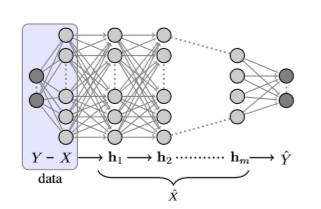
\includegraphics[width=1.0\textwidth]{markovdeep.png}
	\caption{Neuronal Netzwork als Markov Chain}
	\label{fig:Bild1}
\end{figure}

Das ins \ref{fig:Bild4} dargestelle Netzwerk kann als Markov kette betrachtet werden. Wobei jeder Layer h\textsuperscript{n}:1,...,N als ein Zustand einer Markov Kette betrachet werden kann. Wobei der Übergang durch von Informations als h\textsubscript{i} $\rightarrow$ h\textsubscript{i+1} dargestellt werden kann. Da es keine Rekursion gibt und die Information von Input Layer X durch h\textsubscript{arg} zu Output Layer Y durch fließt. Dabei untersuchten sie wie sich die Transinformation I(X;Y) von Input Variable X zu Output Variable Y verhält gegeben durch die Multivariate Verteilung p(X,Y). Dieses Prinzip wird Information Bottleneck Prinziple genannt \cite{bottleneck}. 

\subsubsection{Hypothesen Raum}

Wie in Kapitel Neuronale Netzwerke gezeigt ist das Ziel von ANN haben das Ziel ein Funktion $f*$ zu approximieren. Dabei werden Parameter $\Theta$ eines Models so angepasst, um die Abbildung von y = $f$(x;$\Theta)$ zu approximieren. $f$ bildet also unsere Hypothesen Raum $H$. Die Größe von $\mid H\mid$ wird bestimmt durch die Anzahl von möglichen $f$ welche den Input X auf unseren Output Y abbilden können. Da die Netzwerke letztendlich das Ziel haben eine möglichst niedrigen generalization error zu bekommen. Das heißt die Differenz zwischen Trainingserror und test error sollte möglichst gering bleiben. In einen Experiment zeigeten Zhang und Recht 2016 \cite{hypothesenraum} das Neuronale Netzwerke in der Trainingsphase auch ein Trainingserror zwischen X und zufallsgenerierten Y erlernen können. Natürlich erhöht sich dann der Test error da es keine korrelation zwischen die Zufallsgenerierten Labels und den Labels aus den Validierungsdatensatz gibt.  auf dem validierungsset. Aber ANN können den Trainingsdatensatz komplett auswendig sehen. 
\begin{description}
	\item[Kapazität] The effekitve Kapazität von neuronalen Netzwerken reicht aus den gesamten Datensatz zu speichern.
	\item[Daten]  Even optimization on random labels remains easy. In fact, training time increases only by a small constant factor compared with training on the true labels.
	\item[Random] Randomizing labels issolely adatatransformation,leaving all other properties of the learning problem unchanged\cite{hypothesenraum}.
	
	
\end{description}
Jedes Netzwerk C kann jede Funktion von einer Beispiel der Größe n in der Dimension d representieren wenn für jedes S $\subseteq$ $\mathbb{R}\textsuperscript{d}$ und jede $f$: S $\rightarrow$ $\mathbb{R}$ gibt es Einstellung der Gewichte C sodas C(x) = $f$ für jedes x $\in$ S \cite{hypothesenraum}

\begin{description}
	\item[Theorem] Thereexistsatwo-layerneuralnetworkwithReLUactivationsand2n+d weightsthat can represent any function on a sample of size n in d dimension \cite{hypothesenraum}	
	
\end{description}


\subsubsection{Netzwerkgröße und Trainings Daten größe}

Wie in Hypthesen Raum gezeigt wurde kann ein 2 schichtiges Netzwerk general universel jede $f$ approximieren. Nun ist die Frage wie groß muss mein Netzwerk sein, dass heißt wieviele Schichten um möglichst effizient zu lernen.

\begin{figure}[htbp] 
	\centering
	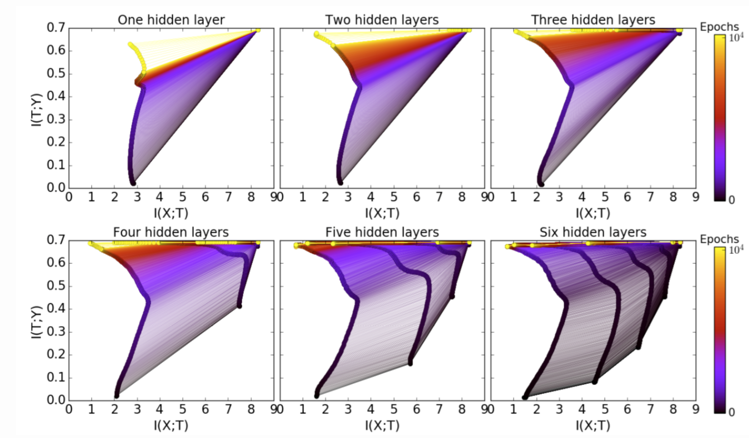
\includegraphics[width=1.0\textwidth]{networksize.png}
	\caption{Größe des Netzwerkes}
	\label{fig:Bild1}
\end{figure}

\subsection{Generative Modelle}

Generative Modelle haben das Ziel eine Wahrscheinlichkeitsverteilungen zu erlernen. Anschließend kann diese als ein Modell genutzt werden und Samples zu erzeugen. Die Modelle können dabei beispielsweise auf ANN oder Markov Chains trainiert werden\cite{Grundlagen}. Im folgenden liegt der Fokus auf ANNs. Ein mögliches Anwendungsbeispiele wären es dem generativen Model, Bilder von bestimmten Objekten zunächst als Trainingsdaten zu geben. Anschließend können von er erlernten hochdimensionalen Wahrscheinlichkeitsverteilung Samples gezogen werden und neue Bilder erzeugt werden, welche nicht im Trainingsdatensatz vorhanden waren. Allgemein gehalten können jegliche Typen von Daten wie Text, Bild oder Audiodateien für generative Modelle herangezogen werden. Es gibt unterschiedliche Typen von generativen Modellen, welche sich vom Aufbau des Neuronalen Netzwerk und der Zielfunktion unterscheiden. Beispiele dafür sind Boltzmann Maschine, Autoencoder oder Deep Belief Networks\cite{Grundlagen}. Diese Arbeit beschäftigt sich mit einen anderen Vertreter, dem Generativ Adverserial Network(GAN). In den letzten Jahren konnte sich das GAN als best practice Ansatz bei den generativen Modellen herausarbeiten was Performancegründe bei der Trainierbarkeit und Qualität der generierbaren Daten zu Grunde liegt\cite{Grundlagen}. 
Die Modelle arbeiten nach der Maximum Likelihood Schätzverfahren(ML-Schätzer) in dem die Parameter $\theta$ dahingegen angepasst werden, dass die unsere beobachtetet Daten am ehesten passen. Man kann ML-Schätzer als Kulback-Leibler(KL) Divergenz darstellen und das generative Modelle das Ziel haben die KL Divergenz zwischen den Trainingsdaten P\textsubscript{r} und den generierten Daten P\textsubscript{g} zu minimieren. In Abbildung \ref{fig:Bild1} ist dieser Prozess dargestellt. Diese Modelle versuchen dann die diese Cost Funktion  
\\
\\
\begin{math}
KL(P\textsubscript{r}|| P\textsubscript{g}])=\int_x P\textsubscript{r}log\frac{P\textsubscript{r}}{P\textsubscript{g}}dx                     
\end{math}
\\
\\
zu minimieren. Wenn nun beide Verteilungen P\textsubscript{r} = P\textsubscript{g} sind, hat das Model sein Minimum Loss erreicht und $\Theta$ muss nicht mehr angepasst werden. Interessant wird es, wenn P\textsubscript{r} $\ne$ P\textsubscript{g}.
Wenn  P\textsubscript{r} $>$ P\textsubscript{g} führt, das dazu dass das Integral schnell gegen unendlich konvergiert. Was dazuführt, das hohe Kosten entstehen wenn die  Verteilung von generativen Modell erzeugt, nicht die Daten abdeckt. Wenn nun  P\textsubscript{r} $<$ P\textsubscript{g} ist, dann bedeutet das, dass x eine niedrige Wahrscheinlichkeit hat aus unseren Trainingsdaten zu kommen aber eine hohe Wahrscheinlichkeit von den Generator erzeugt zu werden. Dann würde sich die KL gegen 0 konvergieren. Was zur Folge hat, dass der Generator Falsch ausschauende Daten geniert aber keine Kosten dafür erzeugt werden und im Umkehrschluss es zu keinen Veränderungen unseren $\Theta$ kommt. Man vermutet das dies der Grund für die Problematiken von generativen Modellen wie Autoencoder und CO sind. Dies ist aber noch kein abgeschlossenen Problem und wird weiterhin erforscht\cite{improvingan}.
Unter GAN werden wir auf dieses Problem erneut aufgreifen und es wird gezeigt inwiefern sich GAN dieses Problem angeht. Generative Modelle gehören zu einem Bereich des unüberwachten Lernens, da keine Labels für die Trainingsdaten gebraucht werden. Probleme welche diese Modelle haben sind beispielsweise, dass Autoencoder zwar mit wenig Trainingsaufwand trainiert werden können jedoch sind die generierten Bilder sehr trüb. Allgemein haben Autoencoder und Co. Vorteile  im Lernen des latenten Raums von Objektlassen, weisen aber Probleme beim Generieren von neuen Daten auf. Da gezeigt wurde das im Deep Learning Bereich die discrimativen Modelle mit Zunahme der Daten stark an Leistung zunehmen. Und GANs Stärke in der Datengeneration in guter Qualität liegt. Kann es seine Vorteil gegenüber den anderen Modellen ausspielen\cite{improvingan}.

\begin{figure}[htbp] 
	\centering
	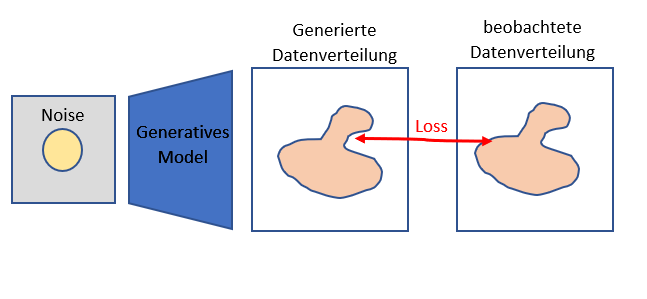
\includegraphics[width=1.0\textwidth]{genmodel.png}
	\caption{Generative Modelle}
	\label{fig:Bild1}
\end{figure}

\subsection{Convolution Neural Networks}

einabuen wie bild bearbeite ist:
https://arxiv.org/pdf/1801.00634.pdf

Convolution Neural Netzworks(CNN) sind eine besondere Art von künstlichen neuronalen Netzwerken, sie sind dafür konzipiert auf Datensätzen zu arbeiten welche in eine Matrix Form gebracht worden sind. Der Input eines CNN können beispielsweise Bilder sein welche durch die Matrix A =
$
\begin{bmatrix}
a_1	& a_1	& \dots	 & a_n     \\
b_1	& b_2 	& \dots  & b_n	  \\
\vdots	& n_n 	& \ddots & \vdots \\
x_1 	& x_2 & x_3	 & x_n
\end{bmatrix}
$
\\\\dargestellt werden. Jedes Element x\textsubscript{ij} stellt einen Pixel eines Bildes da, wobei x\textsubscript{n} $\in$ [0,255] . Die Matrix A\textsuperscript{w$\cdot$b$\cdot$c} stellt w$\cdot$b$\cdot$c = N dimensionale Matrix da. Wobei w die Länge und b Breite des Bildes entspricht. c sind die Farbspektren eines Bildes und sind in einen RGB-Farbraum 3 beziehungsweiße in einen schwarz-weiß Bild 1. Nachdem  der Input eines CNN definiert ist kommt nun der Aufbau. CNN setzen sich aus mehrere Schichten von Convolution Layern zusammen. Ein Netzwerk kann mehrere N-Layer haben. Wobei jeder Layer aus mehreren Convolution oder auch Kernels genannt, zusammengesetzt ist. Ein Aufbau kann aus Abbildung \ref{fig:Bild2} entnommen werden\cite{Grundlagen}.

\begin{figure}[htbp] 
	\centering
	\includegraphics[width=1.0\textwidth]{convol.png}
	\caption{Convolutional Neural Network}
	\label{fig:Bild2}
\end{figure}

Die Kernels, also die einzelnen Filter, von den jeder der N-Layer k besitzt sind K\textsuperscript{n$\cdot$n} Matrizen jedes k\textsubscript{ij} in einem Filter einspricht einen aus der üblichen Neuronalen Netzwerk Architektur bekannten Gewichte. Diese Gewichte werden dann durch den Backprobagation-Algorithmus in der Trainingsphase des Netzwerkes angepasst um den Verlust der Loss-Funktion durch bestimmten des Gradianten zu minimieren. Das durch die Abbildung \ref{fig:Bild2} dargestellte Subsampling ist der Output aus den Convolutional Layern\cite{Grundlagen}. 

Da Input und Kernel unterschiedliche Größen haben und man den gesamten Input mit den Kernel abdecken möchte, bewegt sich der Filter um s Position auf den Input und führt erneut einen Berechnungschritt durch. Dieser Vorgang wird Stride genannt. An jeder Position wird das Produkt von jeden x\textsubscript{ij} des Input und k\textsubscript{ij} des Kernel durchgeführt.  Anschließend werden alle Produkte aufsummiert. In Abbildung \ref{fig:Bild3} ist dieser Vorgang verdeutlicht. Zusätzlich gibt es die Möglichkeit für das sogenannte Zero Padding P. Dabei werden mehrere 0 um die Input Feature Map, am Anfang und Ende der Axen anfügt. Dies ist notwendig wenn Kernel und Input Größe nicht kompatible zueinander sind. Die Anzahl der möglichen Positionen ergeben sich aus Kernel Größe und den Input des jeweiligen Kernel sowie des Strides. Die Output Größ W kann berechnet werden durch W = (W-F+2P)/s+1. Wobei F für die Größe des Kernel steht \cite{conv}.

\begin{figure}
	\centering
	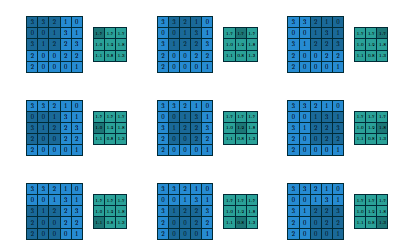
\includegraphics[width=0.8\textwidth]{conv.png}
	\caption{Convolution Beispiel}
	\label{fig:Bild3}
\end{figure}

Um  besser zu verstehen welche Auswirkungen die Anzahl der Kernels in Layer n auf die Größe des Outputs von n und die Anzahl der Kernels in Layer n+1 für den nächsten Layer haben, wird ein Beispiel aufgezeigt. Der erste Layer hat 20 Kernels mit der Größe 7x7 und Stride 1. Der Input A für einen Kernel K ist ein 28x28 Matrix. Der Output aus diesen Filter sind 20 22X22 Feature Maps. Würde der Input ein 28x28x3 Bild mit 3 RGB Channels sein, der Output 60 22x22 Feature Maps. Allgemein kann Convolution Layer als Supsampling gesehen werden und Stride gibt an wieviele Dimensionen bei diesen Prozess pro Convolution Layer entfernt werden soll. Der letzte Layer ist ein fully-connected Layer welcher den typischen Anforderungen von ANN entspricht \cite{conv}.  
\\

Transposed Convolution, auch genannt Fractionally Strided Convolution oder Deconvolution ist eine Umkehrfunktion von der üblichen Convolution. Es verwendet die gleichen Variablen wie Convolution. Dabei wird ein Kernel K mit der Größe N x N definiert der Input I mit der Größe N x N und Stride s = 1. Deconvolution kann wie Convolution angesehen werden mit  Zero Padding auf dem Input.  Das in Abbildung \ref{fig:Bild4} gezeigte Beispiel zeigt einen deconvolution Vorgang mit eine 3x3 Kernel über einen 4x4 Input. Dies ist gleich mit einen Convolution Schritt mit einen 3x3 kernel auf einen 2x2 Input und einer 2x2 Zero Padding Grenze. Convolution ist Supsampling und mit Deconvolution wird Upsampling betrieben. Durch diesen Schritt kommt es zu einer Dimensionserhöhung des Inputs. Die Gewichte der Kernels bestimmen wie der Input transfomiert wird. Durch mehrere Schichten von Deconvolution Layer kann von einer Input Größe NxN auf eine Output Größe KxK, wobei K $>$ N mit Abhängigkeit von Kernel und Stride abgebildet werden\cite{conv}. 

\begin{figure}[htbp] 
	\centering
	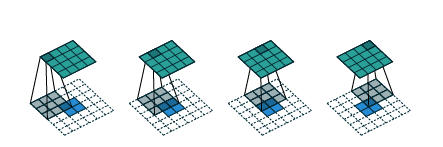
\includegraphics[width=1.0\textwidth]{decon.png}
	\caption{Deconvolution Beispiel}
	\label{fig:Bild4}
\end{figure}
\newpage
\subsection{Generative Adversarial Network}

Ein GAN besteht besteht aus zwei ANN, dem Discriminator D und dem Generator G. Das Ziel des G ist es, Daten x zu erzeugen, welche nicht von Trainingsdaten y unterschieden werden können. Dabei wird eine vorangegangene Input Noise Variable p\textsubscript{z}(z) verwendet, welche eine Abbildung zum Datenraum G(z;$\Phi$\textsubscript{g}) herstellt. Dabei sind $\Phi$\textsubscript{g} die Gewichte des neuronalen Netzwerkes von G. Der Discriminator hat die Aufgabe zu unterscheiden, ob der jeweilige Datensatz von G erzeugt wurde und somit ein fake Datensatz ist, oder von Trainingsdaten y stammt\cite{goodfellow2014}. Die Zusammensetzung zwischen den beiden Netzwerken kann aus Abbildung \ref{fig:Bild5} entnommen werden.
\\
\begin{figure}[htbp] 
	\centering
	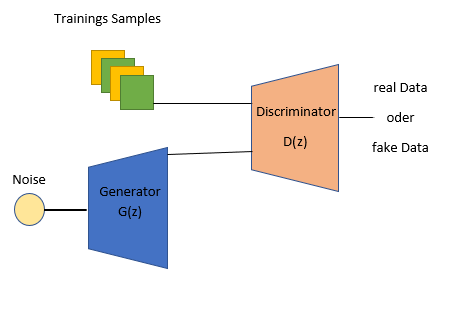
\includegraphics[width=1.0\textwidth]{GAN_GRUNDAUFBAU.png}
	\caption{Generativ Adverserial Network}
	\label{fig:Bild5}
\end{figure}



Der Discriminator ist definiert durch D(x;$\Phi$\textsubscript{d}). Wobei $\Phi$\textsubscript{d} die Gewichte des Descriminators sind und D(x) die Wahrscheinlichkeit ist, dass x von den Trainingsdaten stammt und nicht von p\textsubscript{g}. Die Wahrscheinlichkeitsverteilung für unsere Trainingsdaten ist p\textsubscript{r}.  Im Training werden dann $\Phi$\textsubscript{d} so angepasst, dass die Wahrscheinlichkeit Trainingsbeispiele richtig zu klassifizieren maximiert wird. Und $\Phi$\textsubscript{g} wird dahingehen trainiert die Wahrscheinlichkeit zu minimieren, so dass D erkennt dass Trainingsdatensatz x von G erzeugt wurde. Mathematisch ausgedrückt durch log(1 - D(G(z))). Die gesamte Loss-Funktion des vanilla GAN ist definiert als
\\\\
\begin{math}
min\textsubscript{G} max\textsubscript{D}V(D,G)=E\textsubscript{x$\sim$p\textsubscript{data}(x)}[logD(x)]  + E\textsubscript{z$\sim$p\textsubscript{z}(z)}[log(1-D(G(z))]
\\\\             
\end{math}
diese beschreibt ein Minmax Spiel zwischen G und D. Welches das globale Optimum erreicht hat wenn p\textsubscript{g} = p\textsubscript{r}. Das heißt, wenn die Datenverteilung, welche von G erzeugt wird, gleich der unserer Trainingsdaten ist\cite{goodfellow2014}. Das Training erfolgt durch den folgenden Algorithmus:
\\
\begin{algorithm}[H]
	\For{Anzahl von Training Iterationen}{\For{k Schritte}{$\bullet$Sample minibatch von m noise  Samples z\textsuperscript{(1)},...,z\textsuperscript{(m)}von noise p\textsubscript{g}(z)\\
	$\bullet$ Sample minibatch von m Beispielen x\textsuperscript{(1)},...,x\textsuperscript{(m)}von Daten Generationsverteilung p\textsubscript{data}(x)\\
    $\bullet$ Update den Discriminator zum aufsteigenden stochastischen Gradianten:\\
\begin{math}
\nabla\textsubscript{$\Phi$\textsubscript{d}}\frac{1}{m}\sum_{i=1}^{m}[logD(x\textsuperscript{(i)})+log(1-D(G(z\textsuperscript{(i)})))]
 \end{math}

}$\bullet$ Sample minibatch von m noise Samples z\textsuperscript{(1)},...,z\textsuperscript{(m)} von noise p\textsubscript{g}(z)\\$\bullet$ Update den Generator mit den absteigenden stochastischen Gradianten: \\\begin{math} 
\nabla\textsubscript{$\Phi$\textsubscript{g}}\frac{1}{m}\sum_{i=1}^{m}log(1-D(G(z\textsuperscript{(i)})))\end{math}}
		\caption{Minibatch stochastic gradient descent Training für Generative Adversarial Networks. Die Anzahl der Schritte welche auf den Discriminator angewendet wird ist k }	
\end{algorithm}

Beim Training wird ein stochastischer Minibatch von mehren Trainingsdaten gleichzeitig erstellt. Dies soll dabei helfen, dass der Generator sich nicht auf bestimmte Gewichte fest fährt und auf Trainingssätze kollabiert. So weisen die erzeugten Daten mehr Variationen auf \cite{improvingan}. D wird zunächst in einer inneren Schleife auf n Trainingsätzen trainiert, womit man Overfitting von D vermeiden will, was zur Folge hätte, dass D nur den Trainingsdatensatz kopieren würde. Deshalb wird k mal D optimiert und ein mal G in der äußeren Schleife. 
\newpage
Ein möglicher Aufbau von GAN wird in Abbildung \ref{fig:Bild6} dargestellt. Dies ist das sogenannte Deep Convolution GAN(DC GAN), welches dafür konzipiert wurde auf Bilddaten zu arbeiten. Dabei besteht der Generator aus mehren Schichten von Deconvolution Layern. Welche den Input Noise Variable p\textsubscript{z}(z) auf y abbildet. D besteht aus mehren Schichten von Convolution Layern und bekommt als Input die Trainingsdaten, oder die von G erzeugten Y, und entscheidet über die Klassifikation\cite{dcgan}.

\begin{figure}[htbp] 
	\centering
	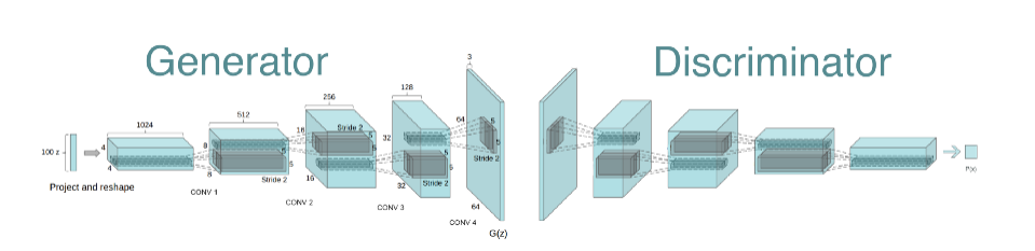
\includegraphics[width=1.0\textwidth]{dcgan1.png}
	\caption{Deep Convolutional GAN}
	\label{fig:Bild6}
\end{figure}



Wie unter Generativen Modellen gezeigt wurde kann das asymmetrische Verhalten der KV Divergenz zu schlechten Trainingsergebnissen führen. Goodfellow \cite{goodfellow2014} zeigte, dass sich die MinMax Loss-Funktion des GAN auch als Jensen-Shannon Divergenz(JS Divergenz) darstellen lässt. Diese ist definiert als\\

\begin{math} D\textsubscript{JS}(P\textsubscript{r}|| P\textsubscript{g}])=\frac{1}{2}D\textsubscript{KL}(P\textsubscript{r}|| \frac{P\textsubscript{g}+P\textsubscript{r}}{2}])+D\textsubscript{KL}(P\textsubscript{q}|| \frac{P\textsubscript{g}+P\textsubscript{r}}{2}])  
\end{math}
\\

wobei P\textsubscript{r} die Wahrscheinlichkeitsverteilung der Trainingsdaten ist und P\textsubscript{g} die des Generators. Huzár \cite{sha} zeigte, dass durch das symmetrische Verhalten der JS Divergenz ein potentiell besseres Trainingsergebnis entstehen kann, im Vergleich zu der KL Divergenz. Damit zeigte weshalb GANs im Vorteil gegenüber anderen generativen Modellen sind.  Abbildung \ref{fig:Bild7} veranschautlicht dieses Konzept.  Der linke Graph zeigt 2 Normal Verteilungen. In der Mitte wird die KV Divergenz der beiden Normal Verteilungen dargestellt.  Rechts ist die JS Divergenz der Beiden dargestellt. Man sieht sehr gut das asymmetrische Verhalten der KV und das symmetrische der JS. Dadurch lassen sich aussagekräftigere Gradianten, bestimmen welche zum Optimieren von D und G benötigt werden\cite{sha}. 
 
\begin{figure}
	\centering
	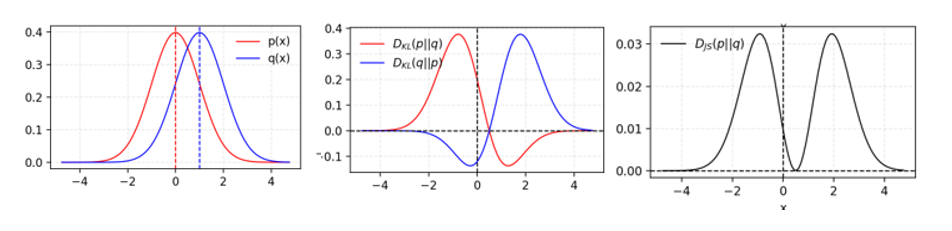
\includegraphics[width=1.0\linewidth]{KLdiv}
	\caption{KL Divergenz und JS Divergenz}
	\label{fig:Bild7}
\end{figure}

\newpage
\subsection{Probleme mit Generative Adverserial Networks}

Wie auch die anderen generativen Modelle haben auch  GANs noch Schwächen bezüglich der Trainingsabläufe und der Qualität der generierten Daten. Im Folgenden wird auf einige Probleme eingegangen.

\begin{description}	

\item[Equilibrium]
D und G betreiben ein MinMax Spiel. Beide versuchen das Nash Equilibrium zu finden. Dies ist der bestmögliche Endpunkt in einen nicht kooperativen Spiel. Wie in dem Fall von GAN wäre das wenn  p\textsubscript{g} = p\textsubscript{r}. Es wurde gezeigt, dass das Erreichen dieses Punktes sehr schwierig ist, da durch die Updates der Gewichte mit den Gradianten der Loss-Funktion starke Schwingungen der Funktion enstehen können. Dies kann zur Instabilität für das laufende Training führen \cite{improvingan}.   
\\
\item[Vanishing gradient]
Dies beschreibt das Problem, wenn D perfekt trainiert ist mit  D(x) = 1, $\forall \in p\textsubscript{r}$ und D(x)=0 $\forall x \in p \textsubscript{g}$. Die Loss-Funktion würde in diesem Fall auf 0 fallen und es gäbe keinen Gradianten, für den die Gewichte von G angepasst werden können. Dies verlangsamt den Trainingsprozess bis hin zu einem kompletten Stopp des Trainings. Würde D zu schlechten trainiert mit  D(x) = 0, $\forall \in p\textsubscript{r}$ und D(x)=1 $\forall x \in p \textsubscript{g}$. Bekommt G kein Feedback über seine Leistung bei der Datengeneration hat er keine Möglichkeit p\textsubscript{r} zu erlernen \cite{improvingan}.
\\
\item[Mode Collapse]
Während des Trainings von GAN kann es dazu kommen, dass der Generator möglicherweise auf eine Einstellung seiner Gewichte fixiert wird und es zu einem sogenannten Mode Collapse führt. Was zur Folge hat, dass der Generator sehr ähnliche Samples produziert \cite{wasserstein}.
\\
\item[Keine aussagegräftigen Evaluations Metriken]
Die Loss Funktion der GANs liefert keine aussagekräftigen Evaluationsmöglichkeit über den Fortschritt des Trainings. Bei  discriminativen Modellen im üblichen Maschine Learning besteht die Möglichkeit Validierungsdatensätze zu verwenden und an diesen die Genauigkeit des Modells zu testen. Diese Möglichkeit besteht bei GANs nicht\cite{metrics}.
\end{description}
\newpage

\subsection{Lösungsansätze für Generative Adverserial Networks Probleme}

Nun werden einige Techniken aufgezeigt, welche die unter Abschnitt Probleme mit GAN genannten Schwierigkeiten angehen und zu einem effizienteren Training führen, damit eine schnellere Konvergenz während des Trainings erreicht wird.
\begin{description}
\item[Feature matching]
Dies soll die Instabilität von GANS verbessern und gegen das Problem des Vanishing Gradient angehen. G bekommt eine neue Loss-Funktion und ersetzt die des üblichen Vanilla GAN. Diese soll G davon abhalten, sich an D über zu trainieren und sich zu sehr darauf zu fokussieren, D zu täuschen und gleichzeitig auch versuchen die Datenverteilung der Trainingsdaten abzudecken\cite{improvingan}.\\

\item[Minibatch discrimination] Um das Problem des Mode Collapse zu umgehen, so dass es nicht zu einem Festfahren der Gewichten von G kommt, wird beim Trainieren die Nähe von den Trainingsdatenpunkten gemessen. Anschließend wird die Summe über der Differenz aller Trainingspunkte genommen und dem Discriminator als zusätzlicher Input beim Training hinzugegeben \cite{improvingan}.\\

\item[Historical Averaging] 
Beim Training werden die Gewichte von G und D aufgezeichnet und je Trainingsschritt i verglichen. Anschließend wird an die Lossfunktion je Trainingschritt die Veränderung zu i-1 an die Loss-Funktion addiert. Damit wird eine zu starke Veränderung bei den jeweiligen Trainingsschritten bestraft und soll gegen ein Model Collapse helfen \cite{improvingan}.\\

\item[One-sided Label Smoothing]
Die üblichen Label für den Trainingsdurchlauf von 1 und 0 werden durch die Werte 0.9 und 0.1 ersetzt. Dies führt zu besseren Trainingsergebnissen. Es gibt derzeit nur empirische Belege für den Erfolg, jedoch nicht weshalb diese Technik besser funktioniert\cite{improvingan}.\\

\item[Adding Noises] 
Noise an den Input von D zu hängen kann gegen das Problem des Vanishing gradienten helfen und das Training verbessern\cite{improvingan}.\\

\item[Use Better Metric of Distribution Similarity] 
Die JS Divergenz von vanilla GAN sorgt für bessere Trainingsergebnisse im Vergleich zu der KL Divergenz von anderen generativen Modelle. Jedoch weißt die JS immernoch Probleme auf.  Es wird vorgeschlagen diese durch die Wasserstein Metric zu ersetzen, da diese bessere Ergebnisse bei disjunkten Wahrscheinlichkeitsverteilungen liefern kann\cite{improvingan}.\\

\end{description}
\newpage

\subsubsection{Conditional Adversarial Networks}

Conditional Adversarial Networks(CGAN) beruhen auf das Grundkonzept von vanilla GAN(vgl. Kapitel GAN). Es wird zusätzlich die extra Information y hinzugefügt. Diese kann jegliche Information sein welche auf x abgestimmt ist. Beispielsweise kann y ein Klassenlabel zu den gelernten P(x) sein. Die Zielfunktion des CGAN ist
\\\\
\begin{math}
min\textsubscript{G} max\textsubscript{D}V(D,G)=E\textsubscript{x$\sim$p\textsubscript{data}(x)}[\log $D$(x|y)]  + E\textsubscript{z$\sim$p\textsubscript{z}(z)}[log(1-D(G(z|y))]           
\end{math}
\\\\    
und beschreibt eine  bedingte Wahrscheinlichkeit das ein Trainingsdatensatz x oder einen Datensatz welcher von den Generator erzeugt wurde von y abhängt \cite{cgan}. 
\begin{figure}[htbp] 
	\centering
	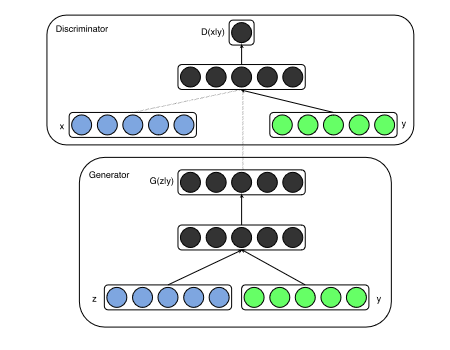
\includegraphics[width=1.0\textwidth]{cgan.png}
	\caption{Conditional Adverserial Network}
	\label{fig:Bild8}
\end{figure}

Ein Beispielhafter Anwendungsfall ist das erlernen von selbstgenerierten Zahlen. Der MNIST Datensatz besteht auch 10000 Handschriftlich eingescannten Zahlen von 0 - 9. Die Daten x können nun während des Training mit den dazugehörigen Zahlenlabels y trainiert werden und anschließend kann der Generator verwendet werden um selbst die gewünschten x zu erzeugen indem y gewählt wird\cite{cgan}. Das Konzept von CGAN wird nun in folgender Arbeit weiterentwickelt um das Ziel zu haben selber Bilder zu verändern. 

\subsection{Image-to-Image GAN}
Image-to-Image GAN(PIX GAN) passiert auf der Grundidee von CGAN bei welche der Generator $\log $D$(x|y)$ lernt und somit eine abhänige Wahrscheinlichkeit von Data x zu einer Zusatzinformation Y. Das Ziel von PIX2PIX ist es ein Input Bild Y zu einen Output Bild $\hat{^y}$ zu verändern. 
\begin{figure}[htbp] 
	\centering
	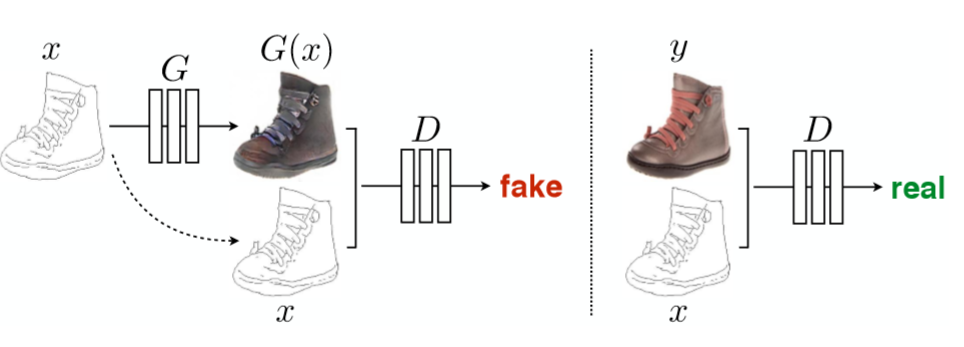
\includegraphics[width=1.2\textwidth]{pix2pix.png}
	\caption{Conditional Adverserial Network}
	\label{fig:Bild2}
\end{figure}


\begin{figure}[htbp] 
	\centering
	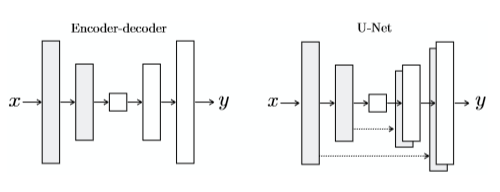
\includegraphics[width=1.2\textwidth]{encoder.png}
	\caption{Conditional Adverserial Network}
	\label{fig:Bild2}
\end{figure}
Die Zielfunktion bleibt die selbe wie beim CGAN besonderheit ergibst sich beim Aufbau des Generators. 
\\\\
\begin{math}
min\textsubscript{G} max\textsubscript{D}V(D,G)=E\textsubscript{x$\sim$p\textsubscript{data}(x)}[\log $D$(x|y)]  + E\textsubscript{z$\sim$p\textsubscript{z}(z)}[log(1-D(G(z|y))]           
\end{math}
\\\\  
Besonderheit ergibts sich beim Aufbau des Generators. Dieses Ähnelt den Aufbau von Autoencodern deren Ziel es ist einen Input zu einen Output Y zu kopieren und dabei zunächst Information zu verringern und anschließend wieder zu erhöhen bis g($f$(x)) = x \cite{Grundlagen}. In fall des PIX2PIX Netzwerkes wird aber das Ziel angestrebt  g($f$(x)) = y zu erlernen und damit eine Bild Transformationen auf die Wahrscheinlichkeitsverteilung P(Y) zu erlangen. 
\cite{imagetoimage}
\subsection{progressiv growing GAN}
\begin{figure}[htbp] 
	\centering
	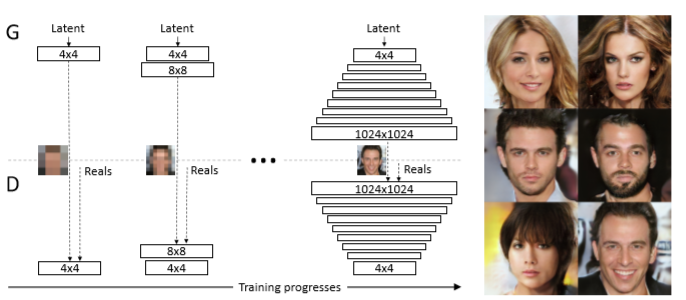
\includegraphics[width=1.2\textwidth]{proggan.png}
	\caption{Conditional Adverserial Network}
	\label{fig:Bild2}
\end{figure}

\cite{progre}
\subsection{3D-GAN}
Das besondere an den 3D Raum im Vergleich zu Normalen 2D Bildern ist die hohe steigerung der Dimension und zu gleich der Hohe Informationsgehalt welcher in 3D Objekten steckt. Das Ziel von 3D-GANS ist es Modelle von Objekten zu erhalten. Dabei wird der latente Objektraum erfasst und soll damit die Wahrscheinlichkeiten für einzelne Objektklassen enthalten. 
\\
Die Architektur des typischen 3D-GAN ist dem vanilla GAN von Goodfellow ähnelt. Durch den Aufbau von 3D-Objekten unterscheidet sich nur die Dimensionalität der einzelnen Layer. Dadurch das 3d Objekte ins Räumliche Verhältnis gestellt werden müssen braucht man eine dritte Dimenson in den Layern welche die Tiefe der Objekte Darstellt. \cite{3d}. 

Die Zielfunktion bleibt die gleiche wie bei den üblichen GANS
\begin{math}
min\textsubscript{G} max\textsubscript{D}V(D,G)=E\textsubscript{x$\sim$p\textsubscript{data}(x)}[\log $D$(x|y)]  + E\textsubscript{z$\sim$p\textsubscript{z}(z)}[log(1-D(G(z|y))]           
\end{math}

\begin{figure}[htbp] 
	\centering
	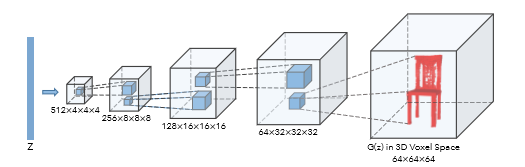
\includegraphics[width=1.2\textwidth]{3dgan.png}
	\caption{Conditional Adverserial Network}
	\label{fig:Bild2}
\end{figure}
\cite{3d}
\section{Methoden}
\subsection{Aufbau}
\subsection{Ergebnis}
\section{Evaluation und Ergebnise}
\section{Zusammenfassung und Diskussion }
Ein GAN besteht aus zwei ANN, dem Discriminator und dem Generator. Das Ziel des G ist es Daten zu erzeugen, welche nicht von Trainingsdaten unterschieden werden können. Der Discriminator hat die Aufgabe zu unterscheiden ob der jeweilige Datensatz von G erzeugt wurde und somit ein fake Datensatz ist, oder von den Trainingsdaten stammt\cite{goodfellow2014}. GANs werden derzeit noch erforscht. Es gibt noch einige offene Fragen, beispielsweise bezüglich der Performance hochauflösender Bilder\cite{ende}. Es wurden in diesem Paper einige Probleme, welche beim Trainieren von GAN auftreten können und mögliche Lösungsansätze, vorgestellt. Es gibt derzeit einige praktische Ansätze, welche in der Anwendung auf GANs zurück greifen. Beispielsweise durch Textbeschreibung eigene Bilder als Output generiert werden \cite{texttoimage}, oder 3D Daten erzeugt werden\cite{3dgan}. GANs finden Anwendung in unterschiedlichen Bereichen des Deep Learnings, da sie als Lösung des Problems angesehen werden, dass Neuronale Netzwerke eine hohe Menge an Trainingsdaten benötigen und GANs dieses Problem durch ihre Fähigkeit, neue Daten zu generieren, umgehen. GANs lernen eine Art "verstecke" Repräsentation von Klassen, was dazu beitragen kann auch Modelle von komplexen Prozessen zu erlernen. Es gibt erste Ansätze bei denen im Reinforcement Learning durch GANs versucht wird Modelle von der Umwelt eines Agenten zu erlernen, welche dann auf Grundlage dieser Modelle Vorhersagen über zukünftige Ereignisse treffen kann\cite{reinforcment}.
\newpage
\listoffigures
\newpage
\listoftables
\newpage
\bibliographystyle{apacite}
\bibliography{mybib.bib}

\end{document}
\end
Alles was hinter \end steht wird von Latex ignoriert...